
How to splitt up the work in paralell tasks










\subsubsection{Parallel improvements} % (fold)
\label{ssub:parallel_improvements}

As we noted in the previous section, the kd-tree build process is by far the most expensive operation, and we would save a lot of time by managing to parallelize this operation. In order to do this, we have to look a bit closer at the different steps of the kd-tree build algorithm.

Steps:
\begin{enumerate}
    \item Find the median of the points along a specified axis. This median point becomes the value of the current node.
    \item Sort all points with lower values than the median to the left of the median, and all the points with higher values than the median to the right.
    \item Perform this algorithm recursively on the left and right set of nodes.
\end{enumerate}

Several strategies can be used to parallelize this code. We can perform the recursive calls as a increasing number of different independent processes. We can also use a parallel algorithm for finding the median in each recursive call. Both strategies can be used in conjunction with each other. The parallel algorithm for finding the median can be used to speed up the early iterations, where we do not have the possibility of calculating several sub-trees in parallel, as well as speeding up the calculation on lather calculations, by utilizing the large number of concurrent threads available in each parallel process.

Different parallel algorithms for finding the median was considered. First we tried to reuse the implementation of bitonic sort. Given a sorted list you can find the median directly, by simply looking at the midmost element of the array. Unfortunately this strategy proved unsuccessful, as re-purposing the bitonic algorithm for such an task proved difficult. We also have the inherent downside of sorting a list in order to find the median, since O(n) algorithms for finding the median exist, compared to the O(n log(n)) time required by sorting.

The existing O(n) algorithms for finding the median is mostly based on a more generic problem, namely selection or
%[kth order statistic algorithms](http://en.wikipedia.org/wiki/Selection_algorithm).
Quick select and radix select to two of the best known selection algorithms in serial. They have both an average time complexity of O(n), witch makes them a good candidates. The difference between then is the constant time penalty. The radix sort have a more exact time complexity of O(bn), where b is the number of bits in each number. While the penalty for quick select is based on n, and if bad pivot elements are chosen the worst case performance is O(pow(n, 2)). We choose to start implementing radix sort based on the results from
%[*Radix Selection Algorithm for the kth
% Order Statistic*](https://github.com/hgranlund/tsi-gpgpu/blob/master/resources/kNN/radix_select.pdf)
. Based on the constant time penalties radix sort would also be the best candidate for large number of elements (n).

The radix select is based on a bitwise partitioning, much like radix sort. In each step, elements are partitioned in two subgroups based on the current bit. Then the subgroup that contains the median is determined, and the search continue in that subgroup until the median is found.

\begin{figure}[ht!]
\centering
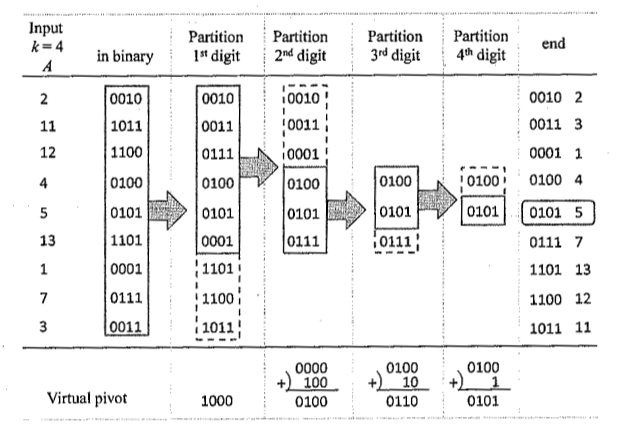
\includegraphics[width=120mm]{../gfx/Radix_select.png}

\caption{An illustration of radix selection.}
\label{fig:radix_select}
\end{figure}

It is hard to use all the parallel power of cuda in this algorithm. The reason is that the problem is divided in three different types; partition one huge list, partition some middle sized list and partition many small lists. This is the reason why we have chosen to use three different implementation of k'th order statistic. The constant time penalties of the two algorithms we have chosen give us a clear indication the radix select is best on large lists while quick select is best on small lists.

Results:
\begin{figure}[ht!]
\centering
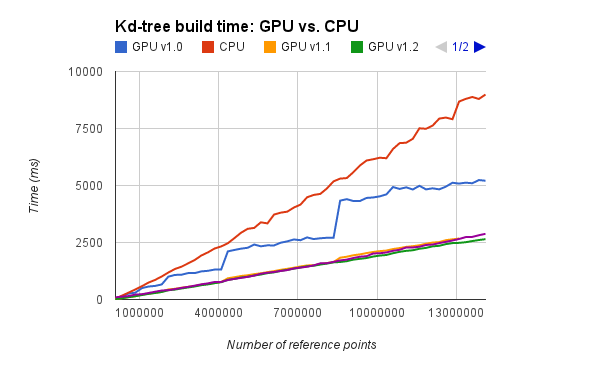
\includegraphics[width=120mm]{../gfx/gpu-vs-cpu-build-time.png}

\caption{GPU vs CPU build time.}
\label{fig:sublime_ide}
\end{figure}

We see that the parallel implementation performs better than the base serial implementation, building a tree of 14 million points in just over 5 seconds, compared to just under 10 required by the serial algorithm. Still we regard this as a quite rough implementation, in need of more tuning to really bring out the speed potential. The potential for parallelizing the workload for the first and last iterations have not been fully developed. This is due to the implementation forcing one version of the radix select algorithm being to work on all problem sizes. This is not optimal for dividing cuda resources, and as a result, we get high penalties when the problem size reaches unsuitable values.

We also see a couple of large jumps in the graph. This happens when the number of elements passes a power of two and the height of the resulting kd-tree increase. The height increase hits the implementation at its weakest.

Tuning the algorithm to alternate between radix select and quick select, eliminates this problem, as is visible in the graph for GPU v1.1. This removes the penalty for calculating the median at unsuitable problem sizes, giving an build time of ~2.4 seconds for 14 million points, compared to the ~9 seconds required by the serial implementation, or the ~5.2 seconds required by the old parallel implementation.

Memory usage:

To analyses the space complexity of the kd-tree build and search algorithm, we have made an theoretical calculation of both algorithms GPU memory consumption, and tested it against results from a GeForce 560ti and a Nvidia grid K520 (amazon web service delved).

It is important to note that the only hard memory limitation is related to building the tree, as a search for N query-points can be performed in several operations. If you e.g. run into memory limitations when searching for pow(10, 8) query-points, you can simply perform two searches on pow(5, 8) query-points to get around the limitation. Loading the pre-built kd-tree on the GPU for searching, and performing one query for a low value of k, will always consume less memory than building the actual kd-tree.

**Kd-tree-build**

The memory consumption for the kd-tree build is only depended on the number of points (n) and the theoretical consumption rate grows linearly as O(36n) subset of O(n).

\begin{figure}[ht!]
\centering
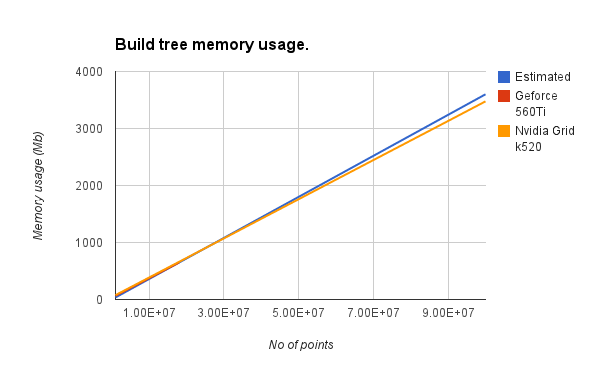
\includegraphics[width=120mm]{../gfx/memory-usage-build.png}

\caption{Memory usage of kd-tree-build.}
\label{fig:memory_usage_build}
\end{figure}

We see that the estimation fit the real consumption almost perfectly, and with this memory model, we can easily estimate the GPU memory requirements for different problem sizes.

Given that a customer wants to perform a knn-search on a point cloud of 100 million, he or she would need a GPU with at least 3.6 Gb of spare memory. Under we have tabulated what maximum problem sizes you would expect to be able to run on a selection of Nvidia graphics cards:

\begin{center}
    \begin{tabular}{ | l | l | p{5cm} |}
    \hline
    Nvidia GPU & Available memory & Maximum problem size \\ \hline
    GTX TITAN & 6144 MB & 1.79E+08 \\ \hline
    GTX 780 & 3072 MB & 8.95E+07 \\ \hline
    GTX 770 & 2048 MB & 5.97E+07 \\ \hline
    Quadro K6000 & 12288 MB & 3.58E+08 \\ \hline
    Quadro K5000 & 4096 MB & 1.19E+08 \\ \hline
    Quadro K4000 & 3072 MB & 8.95E+07 \\ \hline
    Tesla K40 & 12288 MB & 3.58E+08 \\ \hline
    Tesla K20 & 5120 MB & 1.49E+08 \\ \hline
    \end{tabular}
\end{center}

These numbers should be read as rough estimates, as each card is expected to have internal processes requiring an unspecified constant amount of the available memory, therefor lovering the maximum problem size possible to run on these cards in practice. It is also worth to mention that when buying a GPU for GPGPU tasks, other performance characteristics is equally, or more, important.

**Kd-search**

The kd-search is used to query every point against each other. It has a theoretical memory consumption rate at O((40+4k)n) subset of O(kn). The consumption is therefore depended on the number of points (n) and the number of neighbors (k).

\begin{figure}[ht!]
\centering
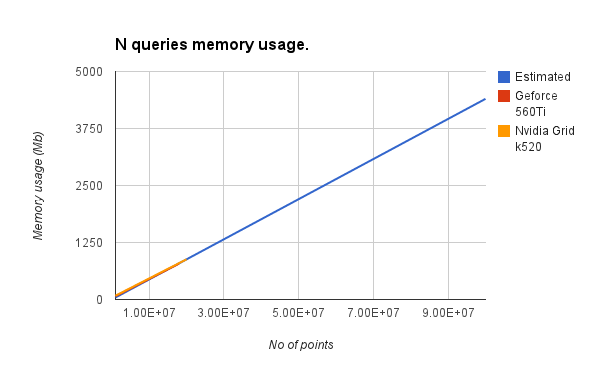
\includegraphics[width=120mm]{../gfx/memory-usage-kd-search.png}

\caption{Memory usage of kd-search.}
\label{fig:memory-usage-kd-search}
\end{figure}

Also in this case our estimation fit the real consumption with a high degree of accuracy.

Further work:
\begin{itemize}
    \item Look at memory optimization.
    \item Improve utiliti methods like: accumulateindex, minReduce.
    \item Forloop Unrolling.
\end{itemize}
